% -*- TeX -*- -*- UK -*- -*- Soft -*-


\part{Evolutionary Algorithms}

\chapter{Evolutionary Algorithms Overview}
\label{chap:EvolAlgoOverview}


\section{Introduction}


``Algorithms that try to find the global optimum can be classified into two categories:
exact, and heuristic. Exact methods guarantee the optimal solution will be found for a given optimization problem, and they are the preferred method if they can solve an optimization problem with an effort that grows polynomially with the problem size. On the other hand, problems that are NP-hard  need exponential effort and even medium-sized problems often become intractable and can not be solved any more using this methods. In order to overcome such limitations heuristic methods can be applied. Heuristics can not guarantee that an optimal solution will be found, but can provide acceptable approximate (also optimal) solutions in a reasonable time. Among the basic heuristic methods we can distinguish between constructive and local search methods. Constructive algorithms generate solutions by adding to an originally empty partial solution components until a solution is complete. On the other hand, local search methods start from an initial solution and iteratively
try to improve it, with a better solution in a defined neighbourhood of the current solution. The following  figure shows an overview of the different optimization approaches''
\cite{Lindquist2017}.


\begin{figure*}[tph]
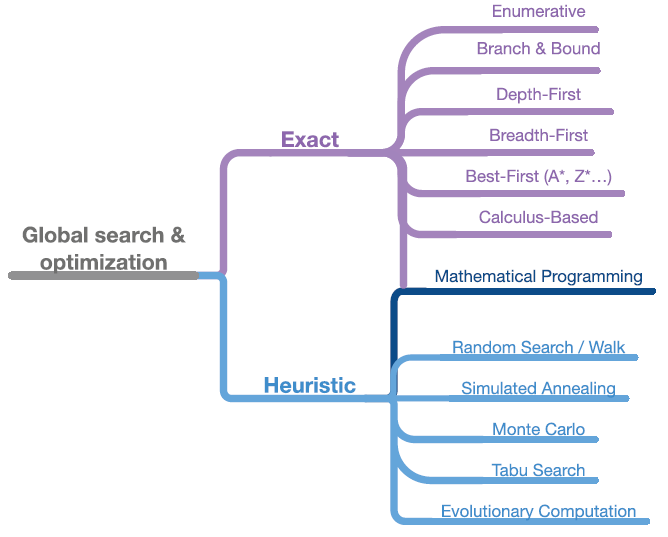
\includegraphics[width=.6\textwidth]{globalsearchmethods}
\caption{Global optimization approaches}
\label{fig:globalsearchmethods}
\end{figure*}


``In artificial intelligence, an \ac{EAlg} is a subset of evolutionary computation, a generic population-based metaheuristic optimization algorithm. An EA uses mechanisms inspired by biological evolution, such as reproduction, mutation, recombination, and selection. Candidate solutions to the optimization problem play the role of individuals in a population, and the fitness function determines the quality of the solutions. Evolution of the population then takes place after the repeated application of the above operators.

``Evolutionary algorithms often perform well approximating solutions to all types of problems because they ideally do not make any assumption about the underlying fitness landscape.  In most real applications of EAs, computational complexity is a prohibiting factor. In fact, this computational complexity is due to fitness function evaluation. Fitness approximation is one of the solutions to overcome this difficulty. However, seemingly simple EA can solve often complex problems; therefore, there may be no direct link between algorithm complexity and problem complexity.''\cite{WikipeadiaEvolutionaryAlgo2019}

Genetic Algorithm was developed by John Holland in 1975. It was shown that it can be used to solve an optimization problem by his student Goldberg, who used genetic algorithms to control gas pipeline transmission. Since then, genetic algorithms have remained popular, and have inspired various other evolutionary programs \cite{Mathur2019}.

Genetic algorithms offer some intriguing advantages and can produce results when the tradition gradient-based approaches fail \cite{Mathur2019}:

A genetic algorithm is like a species. It spawns many singular and unique variations of itself, and those variations are like moth children doomed to be tested against the rigours of the environment. While the environment in real life tests many things about an organism --- strength, intelligence, emotional IQ, fashion sense --- with algorithms, we usually have a single measure of performance: how well an individual instance does with a so-called fitness function. Fitness is a measure of how well an algorithm performs against its predictive goal. 

Given some process, a genetic algorithm would begin by randomly generating a group of inputs to the process, with values that are clearly unsuited to the data at hand. Those randomly generated inputs results in outputs which  are then evaluated in terms of the fitness function to calculate their total error. And the input parameters with the least output error are selected, to create new functions for the next test. Those winning algorithms are recombined; e.g., you mix the parameters of the one with the other. And with several of them, you may introduce mutations; i.e. variations on the fittest parameters, increasing or decreasing them with the purpose of testing the mutated variety.

Spawn, cull, reproduce and mutate: That cycle is repeated until the function surpasses a threshold of  acceptable fitness.

You can use almost any process algorithm within the testing apparatus of a genetic algorithm, which is really just a search algorithm. For example, you can swap in neural networks, and seek the best structure or hyperparameters for the neural net; i.e. those that allow it to learn the most quickly.


Advantages:
\begin{enumerate}
\item They can be used to optimize either continuous or discrete variables.

\item Unlike gradient descent, we do not require derivative information, which also means that there is no need for the fitness function to be continuous and differentiable.

\item It can simultaneously search from a wide sampling of the cost surface.

\item We can deal with a large number of variables without a significant increase in computation time.

\item The generation of the population and calculating their fitness values can be performed in parallel, and hence genetic algorithms are well suited for parallel computers.

\item They can work even when the topological surface is extremely complex because crossover and mutation operators help them in jumping out of a local minimum.

\item They can provide more than one optimum solution.

\item We can use them with numerically generated data, experimental data, or even analytical functions. They specifically work well for large-scale optimization problems.
\end{enumerate}

Despite the previously mentioned advantages, we still do not find genetic algorithms to be a ubiquitous solution to all optimization problems\cite{Mathur2019}: 
\begin{enumerate}
\item If the optimization function is a well-behaved convex function, then gradient-based methods will give a faster convergence

\item The large population of solutions that helps genetic algorithms cover the search space more extensively also results in slow convergence

\item Designing a fitness function can be a daunting task
\end{enumerate}

\section{Overview: Biological }
\TBC{TBC}




\section{Evolutionary Computation}

The information in this section is taken from \cite{DevinSoni2018,skymind2019,Song2016}.

Genes are Basic instructions for building an organism. Genes are located in chromosomes as sequential form, where each gene represents a specific trait of the organism.

The search space contains \lstinline{Populations} that are collections of \lstinline{Individuals} (the equivalent of a biological chromosome).  Each individual (chromosome) is composed of genes, with each gene describing some trait or property.


Genetic and evolutionary algorithms approach mathematical optimization (how do I maximize or minimize a certain value?) in similar ways. What they have in common are ideas drawn from biology: natural selection, reproduction and genetic mutation.

Evolutionary algorithms are a heuristic-based approach to solving problems that cannot be easily solved in polynomial time, such as classically NP-Hard problems, and anything else that would take far too long to exhaustively process. When used on their own, they are typically applied to combinatorial problems; however, genetic algorithms are often used in tandem with other methods, acting as a quick way to find a somewhat optimal starting place for another algorithm to work off of.

The premise of an evolutionary algorithm (to be further known as an EA) is quite simple given that you are familiar with the process of natural selection. An EA contains four overall steps: initialization, selection, genetic operators, and termination. These steps each correspond, roughly, to a particular facet of natural selection, and provide easy ways to modularize implementations of this algorithm category. Simply put, in an EA, fitter members will survive and proliferate, while unfit members will die off and not contribute to the gene pool of further generations, much like in natural selection.

\begin{marginfigure}
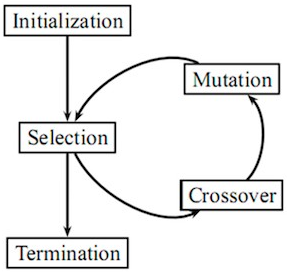
\includegraphics{GA-overview}
\end{marginfigure}

We generally define the problem as such: we wish to find the best combination of elements that maximizes some fitness function, and we will accept a final solution once we have either ran the algorithm for some maximum number of iterations, or we have reached some fitness threshold. This scenario is clearly not the only way to use an EA, but it does encompass many common applications in the discrete case

The common underlying idea behind all evolutionary computation techniques is the same\cite{Eiben2015}:
\begin{enumerate}
\begin{marginfigure}
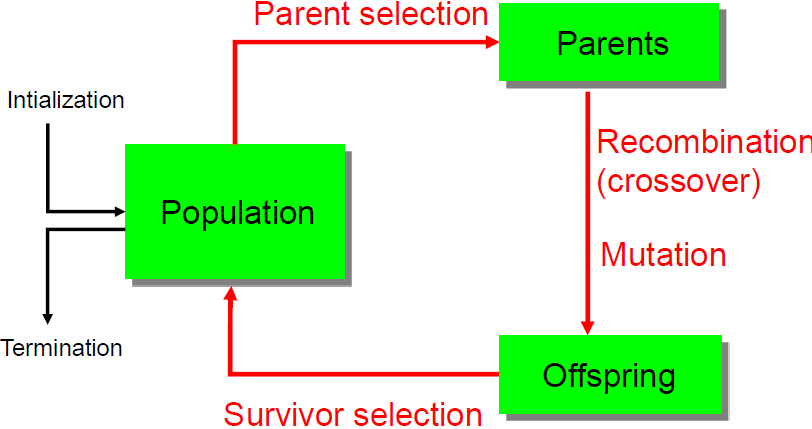
\includegraphics{eibenGA01}
\end{marginfigure}

\item given a population of somewhat random individuals,

\item the environmental pressure causes natural selection (survival of the fittest), which causes a rise in the fitness of the population.

\item Given a quality function to be optimized, we can randomly create a set of candidate solutions, i.e., elements of the function's domain, and apply the quality function as an abstract fitness measure---the higher the better.

\item Based on this fitness, some of the better candidates are chosen to seed the next generation by applying recombination and/or mutation to them. Recombination is an operator applied to two or more selected candidates (the so-called parents) and results one or more new candidates (the offspring/children).

\item Mutation is applied to one candidate and results in one new candidate.

\item Executing recombination and mutation leads to a set of new candidates (the offspring) that compete Based on their fitness (and possibly age) --- with the old ones for a place in the next generation.

\item This process can be iterated until a candidate with sufficient quality (a solution) is found or a previously set computational limit is reached.
\end{enumerate}

In this process there are two primary but opposing forces at work: (1) Variation operators (crossover and mutation) that create diversity and novelty in an increasing population, and (2)  selection of parents and children by fitness, which decreases population and diversity, attempting adaptation/evolution towards an optimised solution.

Note that many components of such an evolutionary process are stochastic. During selection, fitter individuals have a higher chance to be selected than less fit ones, but typically even the weak individuals have a chance to become a parent or to survive. For recombination of individuals the choice of which pieces will be recombined is random. Similarly for mutation, the pieces that will be mutated within a candidate solution, and the new pieces replacing them, are chosen randomly. The randomness brings diversity, whereas the fitness tests try to ensure coherency towards the improved-fit solutions.   In an ill-designed GA the randomness may prevent convergence and even after many generations the solution may still be weak or suboptimal. For this reason it is important to really understand the tools available and make the correct choices when designing the experiment.





\section{Genotype, Phenotype and Genetic Representation}


Eiben describes the \cite{Eiben2015} roles and relationships between genotype and phenotype as follows:
\begin{enumerate}
\item
The first step in defining an EA is to link the problem context to the computation context, that is, to set up a bridge between the two.

Objects forming possible solutions within the problem context are referred to as pheno-types, while their corresponding objects in the computational context are called genotypes.

\begin{marginfigure}
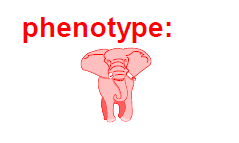
\includegraphics{eibenGA02}
\end{marginfigure}
\item
Phenotypes are the candidate solutions (individuals) existing the problem space (the real-world space).

Fitness evaluation takes place in phenotype space

\item
Genotypes are the experimental solutions (individuals) existing the computational. 
Searching for desired individuals takes place in genotype space.
\begin{marginfigure}
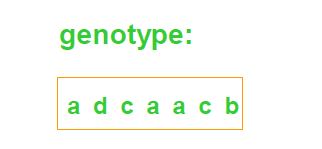
\includegraphics{eibenGA03}
\end{marginfigure}

In order to find the global optimum, every feasible solution must be represented in genotype space.

\item
The representation is the mapping between phenotypes and genotypes. This means designing the genotype data structure to effectively describe the phenotype. 

Sometimes producing the phenotype from the genotype is a simple and obvious process.  Other times the
genotype might be a set of parameters to some algorithm, which works on the problem data to produce the phenotype

\item
The representation must be invertible because the crossover and mutation take place in genotype space, but the individual's genes must be expressed in phenotype space in order to calculate the fitness of the proposed genotype.

Mapping between the two contexts is defined as follows:
\begin{enumerate}

\item
Encoding : phenotype $\rightarrow$ genotype (not necessarily one to one)

\item
Decoding : genotype$\rightarrow$  phenotype (must be one to one)
\end{enumerate}

\end{enumerate}

\begin{figure*}[tph]
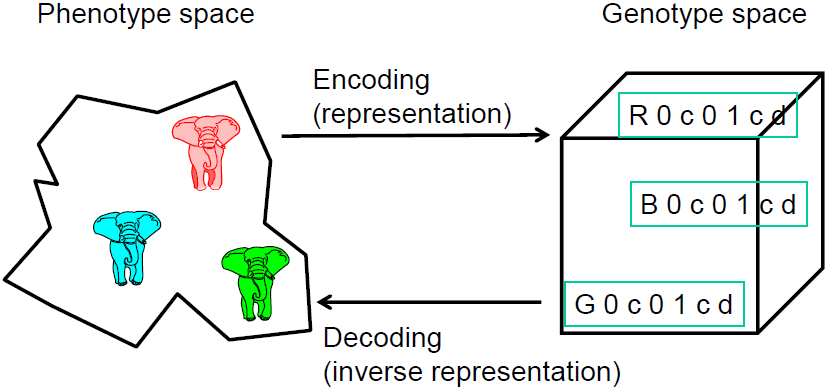
\includegraphics[width=.6\textwidth]{eibenGA04}
\caption{Mapping phenotypes and genotypes}
\label{fig:eibenGA04}
\end{figure*}





\newthought{Binary string encoding} is the original coding used by Holland, and remains most commonly used encoding in examples, but Eiben and Smith believes that most modern GAs use a more sophisticated coding. 
Each chromosome encodes a binary (bit) string. Each bit in the string can represent some characteristics of the solution. Every bit string therefore is a solution but not necessarily the best solution. Another possibility is that the whole string can represent a number. The way bit strings can code differs from problem to problem. Binary encoding gives many possible chromosomes with a smaller number of alleles. On the other hand this encoding is not natural for many problems and sometimes
corrections must be made after genetic operation is completed. Binary coded strings with 1s and 0s are mostly used. The length of the string depends on the accuracy.
In this, (1) Integers are represented exactly, (2)  Finite number of real numbers can be represented, or (3)  Number of real numbers represented increases with string length\cite{Sivanandam2007}.

\newthought{Number string encoding}
Chromosomes can be encoded as strings of values in any base: binary, octal, decimal, ASCII ordinal numbers, etc.  The values in this string have the meaning of magnitude but have no sequence or index meaning.

\newthought{permutation encoding} where chromosomes can be encoded as a string of numbers 
where the number represents and index or location in an ordered sequence.  Most sequences use integers that start at one or zero and increment in contiguous manner up to the end index in the sequence. In most sequences there should be no 'missing numbers' or the same number must not be used twice.
This implies that the crossover and mutation algorithms must comply with the indexing requirements.
For example, mutation and crossover may not result in the same index value being used twice, or end up with missing index values.
Permutation encoding is used in the travelling salesman problem, where the number represents a city and the ordering of the numbers specifies the visiting order.

\newthought{Value string encoding}
Every chromosome is a string of values: from numbers, real numbers or chars to some complicated objects, where the use of binary encoding would be very difficult.  The values can be anything connected to the problem. This encoding produces best results for some special problems. On the other hand, it is often necessary to develop new genetic crossover or mutation operators specific to the problem. 

\newthought{Tree encoding}
This encoding is mainly used for evolving program expressions for genetic programming.
Every chromosome is a tree of some objects such as functions and commands
of a programming language.

\newthought{Approaches to code selection:} 
Early GA work used binary representation with complex decoding and encoding procedures. Furthermore, when executing crossover and mutation, the algorithms must understand the structure encoded in the binary string (if such encoding is used). Modern GA work uses the most appropriate data structure (floating point numbers, structures, etc.), but the requirement still remains that the crossover and mutation algorithms must be able to 
understand and process the genotype.

Corne writes \cite{Corne2018} 
``In common with other optimisation algorithms, most EAs are designed to work with and optimise vectors (or, equivalently, lists or arrays) of decision variables. Solutions to many kinds of problems can be represented, either directly or indirectly, in this form. However, EAs are not limited to working with vectors, and there are often advantages to working directly with representations that are more natural for the problem domain: for example, matrices, trees, graphs, rule sets, etc. Specialised initialisation routines and variation operators are used to randomly create, mutate and recombine instances of the appropriate solution representation.''

Generalised from \cite{Husbands2007} (this was originally written for evolutionary computing for music):
The structures making up the population, the artificial genotypes, are usually strings
of numbers or symbols that represent solutions to the problem at hand. They might be
a string of real numbers that are the parameters or groups of parameters controlling some aspect of the process
Complex encodings involving mixtures of numbers, symbols, rules and other
data structures have also been successfully used. It is also possible to use a fairly simple genotype in
combination with a complex decoding scheme to translate it into the phenotype.
Rather indirect routes to the end goal can be taken. For instance, the genotype may
specify the design of a process, or abstract machine, which is then run to generate the
end product of interest. The genotypes can be of a fixed length
or, where appropriate, they can be allowed to grow and shrink. The great flexibility
available in designing a suitable representation is one of the major advantages over
more traditional methods afforded by the EA framework. However, not all
representations for a given problem will be equally good. In some cases the
representation to use is fairly obvious and straightforward (e.g. a string of numbers
acting as the parameters of a well defined process or design), in others it may not be
so clear. The representation defines the genotype space through which the EA
searches looking for a combination of genes that defines a sufficiently fit phenotype.
If the representation is badly designed the space may become impossibly convoluted
and too difficult to search with any efficiency, rendering the EA useless. 

A good example of how complex genes can be represented is given in \cite{Biles2007}: 
``As every EC practitioner knows, the design of a genetic representation (genotype)
and its mapping into the actual problem domain (phenotype) is critical to the efficacious
use of EC. This is certainly true in representing music. Two representational
dimensions have emerged from the literature, one dealing with how to represent
individual pitches and durations, and the other with how to represent sequences or
other structures in chromosomes.'' Biles then goes on to describe the three approaches to representing note pitch and duration. In the description it is clearly evident that the representation algorithm should not only capture information at the absolute or simplest level (frequency and time). For the purpose of listening to music the relative pitch (i.e., semitones above or below the root signature key) is more relevant and perhaps more useful. A third approach includes the effect of both absolute (the chord root note) and the relative pitch. Each approach has its advantages. Biles then continues to describe \cite{Bilesb2007} how music sections are built up from phrases and measures.  His GenType system has a phrase population of 48 phrase individuals, where each phrase comprises four measure individuals.  The measure population has 64 measure individuals (six-bit string). Each measure individual has eight events, with each event having 16 values (coded in a four-bit string) that represent note selection and duration.
It is evident that this GA has a very complex hierarchical representation, with three evolving populations.


In his PhD thesis on GA optimisation of trading Lindquist \cite{Lindquist2017} codes 19 decision variables structured into a vector of real numbers, where some numbers are integers requiring rounding.  These numbers served as thresholds and weights in the model.  
The first two values corresponded with some aspect of the model, the next three with another aspect,  etc. In other words, the genes were coded as a succession of number sets, of different lengths, adding up to a total of 19 numbers. For all individuals the meaning of a number in the vector at a given index will always be the same. In terms of the model details, the numbers applicable to one aspect of the model always uses some fixed range of indices into the vector. Using bitwise uniform crossover, Lindquist then seems to blend parent individuals' vector values without considering the remaining values in the values' membership to its fixed index range. In other words, if one model required vector values in the range [3:7] he would change variable [5], without considering the values in [3:4,6-7].
\begin{marginfigure}
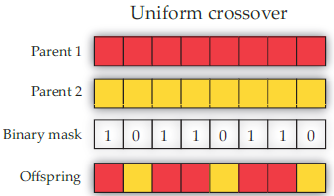
\includegraphics{GA-uniform-CX}
\end{marginfigure}
Mutation is done using the Matlab GA toolbox \textit{adapt feasible mutation} function. My understanding (very scant information available) of this algorithm is that, given that the parameter is an N-dimensional vector, a new vector is added to the present vector such that the magnitude is calculated from a Gaussian random generator and the direction is a randomly generated vector, subject that the variable's constraints are met. If the constraints are not met, new random vectors with (1) ever decreasing magnitudes, and (2) increasingly more directions, are tested until the constraints are met. Meeting the constraints means that the constraints along each dimension are met, but also that the magnitude (linear) constraint is met.

\section{Populations, Individuals, Genes and Alleles}

Starting at the macro level and zooming in to micro level the objects are related as follows:

\begin{enumerate}
\item Population: The population is a multiset of genotype individuals, i.e., repetitions are possible.
The population is the basic unit of evolution, the population is evolving, not the individuals.
Selection operators act on population level, in genotype space.

Example: 
All the words in a book is a population.

\item Individual:
An individual comprises a collection of genes, and can be expressed in genotype space or phenotype space, by its representation rules.

Fitness evaluation takes place in phenotype space, for one individual at a time.

Variation operators (crossover and mutation) act on individual level in genotype space.

Crossover requires two (normally two, but can be more) individuals and produces one or more new individuals Crossover may or may not (elitist algorithm) remove the parents from the population. Watch out for bloating, where the population grows too large.

Mutation requires one individual and produces one individual, where the original individual is destroyed.  

Creation of a chromosome in GA in many cases can be considered as the art \cite{Saenko2015}. In an ideal, the chromosome has to meet two requirements: (1) not to create 'senseless' individuals during the crossing and a mutation, (2) to provide the widest distribution of new descendants and mutations on area of possible decisions.

Example: 
One word found in a book is an individual.

\item Gene:
The gene encodes one (or more) characteristics of an individual. Depending on the nature of the problem a genotype may have more than one instance in the individual, but its meaning is separately significant for each instant. 

Example: 
The letters in a word can be considered the genes the word.


\item Allele:
An allele is one of the possible variational values that a gene can have --- so its relationship to a gene is just like that of a specific value to a variable in mathematics. 
There is an allele to describe a specific variation of the gene.

Example: 
The letters' allele will be the letters in the set called the alphabet.
\end{enumerate}


\section{Steps in Evolutionary Computation}
\subsection{Initialization}
In order to begin our algorithm, we must first create an initial population of solutions. The population will contain an arbitrary number of possible solutions to the problem, oftentimes called members. It will often be created randomly (within the constraints of the problem) or, if some prior knowledge of the task is known, roughly centered around what is believed to be ideal. It is important that the population encompasses a wide range of solutions, because it essentially represents a gene pool; ergo, if we wish to explore many different possibilities over the course of the algorithm, we should aim to have many different genes present.

The DEAP \cite{DEAPDocs2019} overview page makes an important point:  ``Once the types are created you need to fill them with sometimes random values, sometime guessed ones. '' So, if you have some idea of a good starting point, mix your best-guess estimates with  additional random guesses, to start with a blended set.  If your guesses are good, the GA should start better, but the randomness brings in some diversity. \marginnote{In DEAP, construct a best-guess individual with a fitness function and then insert it into the population using \lstinline{pop.append(guess_ind)} or \lstinline{population.insert(0, guess_ind)}. }

\subsection{Selection}
Once a population is created, members of the population must now be evaluated according to a fitness function. A fitness function is a function that takes in the characteristics of a member, and outputs a numerical representation of how viable (goodness) of a solution it is in terms of the problem. Creating the fitness function can often be very difficult, and it is important to find a good function that accurately represents the data; it is very problem-specific. Fitness may be determined by an objective function or by
subjective judgement. The model calculates the fitness of all members, and selects a portion of the top-scoring members, allowing them to pass on their properties or genes to the next generation.

The process of natural selection kills living beings that are unfit for their environments, while those more suited to that environment, by definition, survive and reproduce more prolifically. Thus, those individuals who survived long enough to breed successfully were “selected” by nature, which imposes a rough filter of predators and toxins on the organisms within it, and cuts many threads short. The value these individuals are maximizing is their number of descendents, or copies of their genes circulating in the gene pool.



\subsection{Multiple objective functions}

EAs can also be extended to use multiple fitness functions. This complicates the process somewhat, because instead of being able to identify a single optimal point, we instead end up with a set of optimal points when using multiple fitness functions. The set of optimal solutions is called the Pareto frontier, and contains elements that are equally optimal in the sense that no solution dominates any other solution in the frontier. A decider is then used to narrow the set down a single solution, based on the context of the problem or some other metric.


\begin{marginfigure}
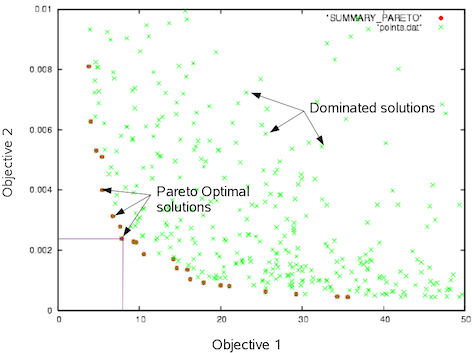
\includegraphics{GA-pareto-frontier}
\end{marginfigure}


\subsection{Genetic Operators}

This step really includes two sub-steps: crossover and mutation. After selecting the top members (typically top 2, but this number can vary), these members are now used to create the next generation in the algorithm. Using the characteristics of the selected parents, new children are created that are a mixture of the parents' qualities. Doing this can often be difficult depending on the type of data, but typically in combinatorial problems, it is possible to mix combinations and output valid combinations from these inputs. Now, we must introduce new genetic material into the generation. If we do not do this crucial step, we will become stuck in local extrema very quickly, and will not obtain optimal results. This step is mutation, and we do this, quite simply, by changing a small portion of the children such that they no longer perfectly mirror subsets of the parents' genes. Mutation typically occurs probabilistically, in that the chance of a child receiving a mutation as well as the severity of the mutation are governed by a probability distribution.

\newthought{Crossover}

When two animals breed, they mix their genes, and those mixed genes are expressed in the child, a new organism. That child represents a genetic experiment in a sense, a test of the world's environment that a species conducts ever so slowly, one brood at a time. If the new genetic mix is successful, the child's genes are propagated to its descendents, and so on to theirs ad infinitum (barring radical changes in the environment). In organisms like humans, reproduction mixes the two halves of a diploid chromosome, one contributed by each parent. Crossover, or recombination, is something different that happens when biological organisms produce gametes (sperm, eggs) whose chromosomes will join in the child. The process of creating gametes is called meiosis, and during meiosis, the chromosomes that are being copied and separated during the cell division swap certain portions of their genes. Bits of genetic information are exchanged for other bits of genetic information stored on a sister chromosome, and an utterly novel sequence of genes is created, which manifests in a more varied species. The builders of genetic algorithms mimic this process to create variation in the parameters of the algorithms tested, swapping digital bits instead of genetic ones.

Crossover is the process of taking more than one parent and producing offspring from them.
By recombining portions of good individuals, the GA could perhaps create a better individual.
Various methods for combining the parents (One-point Crossover, Edge Recombination, and many more).

Crossover techniques can follow simple rules (as described above) or it can be sensitive to the context. 
Biles describes \cite{Bilesb2007} the following crossover algorithm that makes sense in music: 
\begin{lstlisting}
At each of the seven potential crossover points (in 4/4 time)
     Compute horizontal intervals that would result in both children
     Return the smaller interval as ``fitness'' for that point
If more than one crossover point has the same fitness
    If breeding two of GenJam's measures
        Select crossover point closest to the centre of the measure
    If breeding a GenJam measure with a human measure
        Select crossover point that maximizes the human's contribution
Perform crossover at selected point.
\end{lstlisting}
Biles has similar crossover algorithms at phrase level. To some extent he has done the perfectly correct thing by  implementing some of the rules followed by composers, into the crossover algorithms.
Clearly, this algorithm has very strong input from the context and also from an external rule set for legal or acceptable crossover.  It would seem that if the crossover follows some intelligent rules (in contrast to random bit switches) the GA should reach its goal quicker and perhaps more accurately.

\newthought{Mutation}

As genes are copied and relayed from one generation to the next, mutations creep in. The genes' order might be misread, and one piece of genetic information substituted for another. From one perspective, mutations look like mistakes, and many indeed lead to the death or impairment of the organism. From another perspective, mutations allow a species to explore the space of all possible genetic combinations, and in so doing, they show whether or not a totally new combination of genes is better than anything that was born before. Mutations ensure diversity, which itself is a hedge that populations make against disease. Mutations also support the continued exploration of a large combinatorial (and undifferentiable) problem, which is especially important given that environments change,1 and those changes can kill off a stagnant and homogeneous species, or favour a novel mutation in its ranks.

Genetic variation emerges due to damaged DNA, transposition, errors in DNA replication, broken DNA repair processes and recombination; in algorithms, it results from deliberate point mutations in parameters (e.g. random-number generation), as well as crossover.

With crossover, offspring can get good traits of its parents, but they can't get traits that parents don't possess.
Offspring can have traits which their parents don't have by mutation.  Mutation encourages genetic diversity among individuals and
attempts to avoid getting stuck in local minima in the search space.

In Holland's original GA work, the genotypes were bit strings and mutation meant changing single bits randomly. 
This naive approach can be made more sophisticated on many levels.
 If the genotype representation only contains bit-structured data such as float numbers, changing a bit might not have the intended meaning or it may destroy the number completely.  In this case, a valid mutation would be to change the floating point number by some arithmetic operator or randomly replace it with another number. The newly mutated number must comply with the range of legal values for the gene.
 A higher level mutation may apply a context-dependent mutation, such as conditional on another gene.  If the other gene has a certain value the mutation must comply with some condition, as Biles did for real-time music evolution as described in \cite{Bilesb2007}.
\marginnote{Biles describes the following mutations that make sense in music: transpose down, reverse, rotate, sort new notes up, sort new notes down, invert, invert reverse, sequence phrase, lick thinner, and orphan phrase. These mutation are some of the tools available to the composer to create meaningful music, so it only makes sense to use these as mutation operators.}

\subsection{Termination}
Eventually, the algorithm must end. There are two cases in which this usually occurs: either the algorithm has reached some maximum runtime, or the algorithm has reached some threshold of performance. At this point a final solution is selected and returned.

\subsection{Genetic and Evolutionary Algorithms}




\TBC{TBC}


\subsection{Maximising or Minimising?}

Some real-world problem objectives are to achieve a maximum in the outcome The problem with optimizing towards a maximum in a population with many large values is that the large values will completely swamp (and therefore hide) any smaller or poor performing values. 

\begin{lstlisting}
(1) Maximising towards +infinity:
[   1. 1000. 1000. 1000. 1000. 1000. 1000. 1000.] 
mean=875.125 max=1000.0
\end{lstlisting}

Taking the inverse values, the mean value (0.13) is now significantly affected by the poor performing individual, and less so by the well performing individuals:
\begin{lstlisting}
(2) Minimising the inverse towards zero:
[1.    0.001 0.001 0.001 0.001 0.001 0.001 0.001] 
mean=0.13 max=1.0
\end{lstlisting}


The Matlab documentation and Wikipedia \cite{wikipediaMultiobjectiveoptimization2019} propose to negate the value and then maximise this negated value (find the value closes to zero). This would work where a single value is sought, such as the maximum of a function.
This approach will not work when the ensemble performance is required, such as when acceptable performance from all samples are required, compared to he good performance of a single sample.

\begin{lstlisting}
(3) Minimising the negative towards zero:
[   -1. -1000. -1000. -1000. -1000. -1000. -1000. -1000.] 
mean=-875.12 max=-1.0
\end{lstlisting}

The data above demonstrates the problem with maximising optimisations using a simple fitness measure. It is evident that the best choice depends on the task at hand.

\begin{enumerate}
\item Maximising $f(x)$ towards $+\infty$ causes the (undesired) smaller outcomes to disappear in the mean and the maximum of the data set.  Neither the mean nor the max functions will optimise the low performers.

\item  Minimising $f(1/x)$ towards 0 causes the (undesired) smaller outcomes to rise and have a much stronger effect than the outcomes of the well-performing outcomes (which disappears towards 0). Either the mean or the max functions will optimise the low performers.

\item  Minimising $-f(x)$ towards 0 only works when using the minimise-towards-zero function on the individual values, because the mean function swamps the low performer outcomes with large negative values. The mean of all values should not be used in this case.

\end{enumerate}

To find the single maximum value of a function, optimise the single values (not the mean).   For ensemble performance, use (2), the inverse method, and the mean of the values.

So the objective should be to optimise towards the best fit (approaching zero value), so that the well performing solutions will have  lower impact on fitness.  It is proposed that most  real-world optimisations should employ some 'inverted' fitness measure. The simple mathematical reciprocal may not be the best choice, some work may be required to find a good measure.
Irrespective of the exact mapping the effect should be inverse-related.
On the assumption of an inverse fitness measure, we define the best match to approach zero, either on mean value or singular value.


%# to investigate the minimising options
%
%a = np.ones(8)*1000
%a[0] = 1
%b = a
%print('(1) Maximising towards +infinity:')
%print(f'{b} \nmean={np.mean(b)} max={np.max(b)}\n')
%
%print('(2) Minimising the inverse towards zero:')
%b = 1 / a
%print(f'{b} \nmean={np.mean(b):.2f} max={np.max(b)}\n')
%
%print('(3) Minimising the negative towards zero:')
%b = - a
%print(f'{b} \nmean={np.mean(b):.2f} max={np.max(b)}\n')



\section{Strategies and Pitfalls}

GAs (Genetic Algorithms) and GP (Genetic Programming) are investigated
for finding robust Technical Trading Strategies (TTSs). TTSs evolved with
standard GA/GP techniques tend to suffer from over-fitting as the solutions
evolved are very fragile to small disturbances in the data. The main objective
of this thesis is to explore optimization techniques for GA/GP which
produce robust TTSs that have a similar performance during both optimization
and evaluation, and are also able to operate in all market conditions
and withstand severe market shocks \cite{Lindquist2017}.




We employ an elitist $\mu + \lambda$ evolutionary process where from $\mu$ parents we
generate $\lambda$ offspring and the best individuals from both $\lambda$ and $\mu$ form the
population of the next generation.  $\mu + \lambda$ has the advantage of not losing
the best solutions during evolution as they are never replaced by inferior
individuals \cite{Lindquist2017}.


If the genes are floating point and initially randomly valued, any uniform crossover swapping will not change the randomness of the chromosomes is maintained and no new information is added to the chromosome.
The problem with these point crossover methods is that no new information
is introduced: each continuous value that was randomly initiated in the initial
population is propagated to the next generation, only in different combinations.
Although this strategy worked fine for binary representations, there is
now a continuum of values, and in this continuum we are merely interchanging
two data points. These approaches totally rely on mutation to introduce
new genetic material.
The blending methods remedy this problem by finding ways to combine
variable values from the two parents into new variable values in the offspring.
A single offspring variable value, $p_{new}$, comes from a combination of the two
corresponding offspring variable values $p_{\text {new}}=\beta p_{m n}+(1-\beta) p_{d n}$,
where $\beta$ is a random number on the interval [0,1] and the two genes are the nth variable in the father and mother chromosomes.
When $\beta$ = 0.5 the result is an average of the variables of the two
parents.This method is demonstrated to work well on several interesting problems.
These blending
methods effectively combine the information from the two parents and
choose values of the variables between the values bracketed by the parents;
however, they do not allow introduction of values beyond the extremes
already represented in the population. To do this requires an extrapolating
method.  For more information see Chapter~3 in \cite{Haupt2004}.




%A place-holder is commonly called a variable, a locus (plural: loci), a position, or in a biology-oriented terminology a gene. An object on such a place can be called a value or an allele. Alternatively, chromosomes contain genes, which are in (usually fixed) positions called loci (sing. locus) and have a value (allele)

%One of the possible advantages of evolutionary algorithms over neural networks, at least for some problems, is that they do not require gradients; i.e. evolutionary algorithms can explore a parameter space in order to decrease error without depending on backpropagation and differentiation that relates those weights to the error. This is important in environments where reward signals may be sparse and dependencies remote, or when you're dealing with discrete parameters, similar to genes, rather than continuous curves.
